\newpage \flushleft{\huge{\bf Chapter 1}}
\section{INTRODUCTION}

%-----------------------------------------------------------------
% IMPORTANT
%-----------------------------------------------------------------
\pagenumbering{arabic}  % Only here. Don't put in subsequent chapters.
%-----------------------------------------------------------------


\subsection{Hexagonal Boron Nitride and Graphene}


Since the successful isolation of graphene from graphite by the Scotch tape method reported by Novoselov and Geim in 2004 (\cite{novoselov2004electric}) the research on graphene and two-dimensional (2D) materials has been exploded due to their unique, peculiar and fascinating low dimensional structures and properties in contrast to those of their bulk and other dimensional counterparts (\cite{xu2013graphene}). In the past few years, tremendous attention has been paid to 2D hexagonal boron nitride (hBN), which is by itself an electrical insulator with an ultra-flat surface and a highly stable structure. Although hBN is electrically insulating, it can well be tuned by several strategies for differing properties and functionalities, such as by doping, substitution, functionalization and hybridization (\cite{zhang2017two}). It can also be used to tune the carrier mobility of other two-dimensional materials, such as graphene, $ \text{MoS}_{2} $ and BP, when properly synergized together due to the reduced coulomb scattering and excellent interface properties, and to protect these active materials from contamination, oxidation, and thermally/ electrically induced degradation (\cite{zhang2017two}). Driven by the anticipated huge technical potential, single- and few-layer hBN nanosheets have been successfully developed and investigated, which have indeed been shown to exhibit abundant appealing properties for technologically demanding applications, such as DUV photonic devices (\cite{jiang2014hexagonal}) dielectric tunneling (\cite{hui2016use}), power devices (\cite{constantinescu2016multipurpose}), electronic packaging (\cite{bao2016two}), fuel cells (\cite{oh2014enhanced}), and biomedicines (\cite{chimene2015two}). 2D-hBN nanosheets, which are s$\text{p}^{2}$-hybridized 2D insulators, are structural analogues of graphene with sublattices being occupied by equal numbers of boron and nitrogen atoms alternately arranged in a honeycomb configuration. The hexagonal crystal structure of hBN with crystallographic parameters of a = 0.250 nm and c = 0.666 nm and the interlayer spacing of 0.333 nm enable excellent interaction with graphene, and hence it has great potential for various device applications. Similar to graphene, the weak van der Waals interaction dominates between the different hBN planes, which are covalent-bonded within the plane and are highly polarized because of the high asymmetry of the sublattices, resulting in a large band gap (5–6 eV). As the weak interlayer interaction in hBN, van der Waals forces and electrostatic forces are largely responsible for anchoring the interlayer distance and dictating the optimal stacking modes.

The characteristic resistance to oxidation and corrosion makes 2D-hBN a suitable candidate as a gate dielectric and capping layer to protect the active material element and device from structural deformation and chemical degradation (\cite{li2016atomically}). Additionally, due to being electrically insulative with a wide bandgap of 5.97 eV and optically transparent, 2D-hBN can be applied as a barrier and active layer to implement the tunneling devices and tune the carrier dynamics and optical properties. Its high thermal stability (up to 1000 °C in air and 1400 °C in vacuum) (\cite{li2014strong}), superior thermal expansion coefficient (1-layer, 2-layer and 9-layer correspond to 3.41 102 , 3.15 102 and 3.78 102 c$\text{m}^{-1}$ $\text{K}^{-1}$ , respectively) and conductivity (484 W $\text{m}^{-1}$ $\text{K}^{-1}$ ) as well as excellent mechanical strength (elastic constant of 220–510 N$\text{m}^{-1}$ and Young’s modulus 1.0 TPa) (\cite{kumar2016optimised, wang2016fabrication}) further benefit 2D-hBN in various other applications. The stability and performance of 2D-hBN-based devices are of course highly dependent on the quality of 2D nanosheets, which consequently requires a careful control of the synthesis process. This has indeed stimulated new strategies and innovation in controlling the material growth processes and understanding the formation mechanisms (\cite{wang2016fabrication, bao2016synthesis}). Despite the great progress achieved so far, the current research into 2D-hBN still faces three major challenges: (a) growth of large-scale hBN with controlled layer quality and corresponding transfer technique, (b) integration of 2D-hBN into other nano-materials or nano-devices, (c) effective modulation of electronic structures by other strategies (including energy bands and charge carriers) in 2D-hBN (\cite{nam2014graphene}).
Graphene is a single layer of carbon atoms that are connected in hexagonal lattice to form honey comb structure. Thanks to its excellent thermal, mechanical, structural and optical properties (\cite{lee2008measurement, calizo2009raman, ahn2014things, balandin2008superior}), graphene has gained a huge attention of research scientists. These outstanding properties are shown by graphene because of its unique electronic structure and hexagonal arrangement of carbon atoms in lattice (\cite{neto2006drawing}). Graphene could be combined with other materials to synthesize graphene reinforced metal matrix composites (Gr-MMCs). Such composites take the benefit of extraordinary properties of graphene and, therefore, also exhibit excellent properties.

Carbon atom has electronic configuration of 1$\text{s}^{2}$ 2$\text{s}^{2}$ 2$\text{p}^{2}$. When two carbon atoms combine together, s$\text{p}^{2}$ hybridization occurs because one election from 2s orbital transfers to 2p-orbital thereby bringing three orbitals 2s, 2px and 2py to same energy level (\cite{littlejohn2013electrical}). This enables single carbon to form strong covalent bond with three carbon atoms thus forming a hexagonal lattice (\cite{tiwari2016magical}). The C-C planar sigma bond has bond length of 0.142 nm imparts graphene exceptionally high planar strength (\cite{huang2011graphene}). Excellent functional properties of graphene are imparted by unhybridized 2pz orbitals which form delocalized electronic clouds over the hexagonal ring (\cite{agarwal2018carbon}). Due to unique atomic structure and electronic interactions, Dirac cones are formed at each edge of hexagonal ring. Graphene has zero bandgap nature because of these Dirac cones (\cite{abbott2007graphene}). High charge carrier mobility of graphene results in its excellent thermal and electrical conductivities because of the presence of massless Dirac fermions and ballistic charge transport (\cite{bolotin2008ultrahigh}).
As mentioned earlier, the properties of graphene depend on the structure of carbon lattice and functional groups associated with each of its derivatives. Graphene derivatives can be classified into several types based on layers number, functional groups and crystallographic structure (\cite{geim2009nature}). On the basis of number of layers, the graphene derivatives are categorized into single-layer graphene, few layered graphene (FLG), multilayered graphene (MLG), and graphene/graphite nanoplatelets (GNPs) (\cite{kauling2018worldwide}).  In addition, graphene has excellent mechanical properties; the tensile strength of graphene measured by the experiment is about 130 GPa (lee2008measurement), which is 100 times that of ordinary steel; its fracture strength can reach 42 N/ $\text{m}^{2}$, about 200 times that of steel (lee2008measurement). At the same time, the elastic elongation of graphene is also higher than that of all other crystals, and the elongation rate can reach 20\%; the elastic constant of graphene is 1 ~ 5 $N4\text{m}^{-1}$, and the Young's modulus is as high as 1.02 TPa (\cite{lee2008measurement}). These excellent properties of graphene materials generated huge interests in the applying it in a myriad of device and in the fields of thermoelectric and optoelectronic devices, ultrastrong paper-like materials, electrocatalysts, novel composite materials, energy conversation materials, and so on. In this dissertation, the potential of graphene to reinforce metals and alloys will be focused.

Graphene and hBN materials hold a prominent position among nanomaterials due to their colossal potential to improve the properties of metals and alloys [xxx]. In order to benefit from their atypical functional and structural properties, scientific community continues to research on developing MMCs reinforced by graphene and hBN [xxxx]. Despite of all the research that has been performed on this topic, there are still some gaps which need to be filled and true potential of graphene or other 2D materials is yet to be explored. The fabrication techniques to develop 2D reinforced metal matrix composites (MMCs) are continuously flourishing; efficient and economical methods need to be introduced for the fabrication of 2D materials reinforced MMCs.



\subsection{2D Materials-based Metal Matrix Composites}


Metal-matrix composites are metals or alloys that incorporate particles, whiskers, fibers, or hollow micro balloons made of a different material, and offer unique opportunities to tailor materials to specific design needs (\cite{mortensen2010metal, sidhu2016metal, miracle2005metal}). These materials can be tailored to be lightweight and with various other properties including: high specific strength and specific stiffness, high hardness and wear resistance, low coefficients of friction and thermal expansion, high thermal conductivity, and high energy absorption and a damping capacity (\cite{miracle2005metal}). In addition to these properties, new MMCs are being developed with self-healing, self-cleaning, and self-lubricating properties, which can be used to enhance energy efficiency and reliability of automotive systems and components (\cite {macke2012metal}). Since the last three decades, metal matrix composites (MMCs) have been intensively studied in order to develop high performance materials exhibiting distinguished properties.

MMCs can be divided into three different types in terms of the reinforcement, which are fibre-, particle- and flake-reinforced MMC (\cite {clynetw1993anintroductiontometalmatrixcomposites, ibrahim1991particulate, chawla2012metal}). Fibre-MMC consists of reinforcement fibres and metal bulk in which the typical fibres are boron, SiC, Al2O3 and graphite (\cite {chou1985fibre}). The reinforcement fibres are used for adhesion, stress transfer and thus effectively improve the tensile strength of the composites (\cite{shirvanimoghaddam2017carbon}). The fibre-reinforced MMCs are usually used as structural materials with high strength and elastic modulus (\cite {vijayaram2006fabrication}). The particles used in particle-MMC are typically SiC, $ \text{MoS}_{2} $ and h-BN particles (\cite {chawla2001mechanical}). These composites have less tensile strength and elastic modulus, while the hardness and stiffness are higher compared with fibre-MMC (\cite {zhang1995wear}). Therefore, particle-MMC is often used to enhance the tribological properties of composites (\cite {chawla2001mechanical}). As for flake-MMC, graphene is the most representative reinforcement component (\cite {wang2012reinforcement}). With the aid of the excellent mechanical properties and unique pristine 2D structure of graphene, the tensile strength and elastic modulus could be extensively increased in two directions, other than the one-direction case of fibre reinforcement (\cite {kumar2014graphene}).

The performance of MMC mainly depends on the selection of reinforcement materials for improving the mechanical and tribological properties (\cite {hg2017tribological}). In the case of traditional MMC materials, the reinforcement materials include microparticles, fibres and crystal whiskers (\cite {chawla2001mechanical}). The recent development of 2D materials, including graphene, $ \text{MoS}_{2} $, WS2 and h-BN, which have naturally high strength and strong interfacial bonding, leads to the opportunity for tailoring the MMC materials in nanometre-scaled range with improved performance (\cite {hg2017tribological, kasar2018graphene, nieto2017graphene, nautiyal2019copper, xiao2017tribological}). Many studies on these composites specifically address the uniform distribution problem of these 2D materials in a metal matrix, followed by the presence of porosity (\cite {hg2017tribological, kasar2018graphene}). On the other hand, the huge density difference between 2D materials and metal matrix, high interfacial contact area, and reaction activity of 2D materials will also lead to poor interfacial bonding between these 2D materials and metal matrix (\cite {kasar2018graphene, takeda2017cu}). Therefore, it is essential to improve the dispersion properties of graphene, $ \text{MoS}_{2} $, WS2 and h-BN in metal matrix systems for enhanced mechanical properties of MMC. This review will first summarize the fabrication methods of MMC and the challenges in the fabrication process thus far. The effects of the reinforcement component on mechanical properties of MMC were presented, followed by the analysis of their mechanical and tribological properties.

\subsection{Current Challenges for Fabricating 2D Materials-Based MMCs}

Proper dispersion of graphene/hBN in a metal matrix is essential to achieve MMCs with desired properties. The incorporation of graphene/hBN should be carried out such that there is no agglomeration, uniform distribution, good interfacial attachment, and proper structural integrity. Severe agglomeration of graphene is one of the main problems to fabricate graphene reinforced metal matrix composites (Gr-MMCs) (\cite {hu2016laser}). Agglomeration occurs as a result of Van der Waal’s forces between graphene sheets (\cite {zandiatashbar2012mechanical}). Commonly, Gr-MMCs are fabricated using GNPs and MLGs which contain 10~100 layers of carbon atoms (\cite {nieto2017graphene}). As a result, there is a big difference in properties between these multilayer graphene derivatives a single layer graphene. With the multilayer graphene derivatives, agglomeration is one of the basic challenges because this can unavoidably lead to the large porosity in structure. This may in turn cause premature failure of the composite because of premature crack initiation and propagation (\cite {song2016microscopic, chu2014enhanced, li2014highly}). Another serious concern is the poor dispersion of graphene in metal matrix (\cite {chu2018anisotropic}) which leads to the poor properties of MMCs. Inhomogeneous distribution of graphene results in increase in porosity and decrease in yield strength, thermal, and electrical conductivities of composite (\cite {asgharzadeh2017synthesis}). Furthermore, in order to ensure good properties of MMCs, wettability between the reinforcement material and metal matrix is also an important parameter to consider. If the wettability is low, there is weak interface between enforcement material and metal matrix and hence composite will demonstrate poor properties (\cite {kauling2018worldwide}). As mentioned earlier, graphene possesses extraordinary properties only due to its unparalleled electronic and chemical structure. So, in order to avail maximum benefits from the outstanding properties of graphene in MMCs, it is important that its chemical and electronic nature of structure is preserved. Unfortunately, conventional methods of fabricating MMCs impose harsh processing conditions and hence cause damaging the actual properties of graphene. Various types of deteriorations include thermal decomposition of graphene, high defect density in graphene sheets and lateral size reduction etc. (\cite {nieto2012synthesis, perez2014microstructural}). These defects not only miserably affect the thermal and electrical behavior of MMCs but also result in premature failure (\cite {chu2018largely}). It must be noted here that the hBN is structurally analogous to graphene having almost all comparable properties to graphene. In this perspective, the challenges towards the development of hBN reinforced metal matrix composites (hBN-MMCs) are the same as towards the development of Gr-MMCs.  In the coming section, we therefore present various processing techniques to fabricate Gr-MMCs with their advantages and limitations. 

\subsection{Fabrication Methods}

Incorporation of graphene in metal matrices has been carried out by utilizing various techniques since last decade (\cite{nieto2012synthesis, hu2016graphene, kumar2014graphene}). The main focus was to address the aforementioned challenges in the fabrication of Gr-MMCs. The processing techniques can be broadly classified 
into following classes.

\begin{enumerate}
\item Mechanical alloying (MA)
\item Semi powder metallurgy (SPM)
\item Molecular-level mixing (MLM) 
\item In-situ growth
\end{enumerate}

The forthcoming section illustrates an overview of each processing technique so that we could get familiarization about their scope.


\subsubsection{Mechanical Alloying (MA)}

MA involves the mixing and blending of graphene and metal powders. This technique is widely being employed for fabrication of Gr-MMCs (\cite{kim2014multi, dutkiewicz2015microstructure, borkar2015excellent, yalccin2019enhancement, salvo2019enhanced}). Mixing and blending are mostly carried out by using ball milling technique which not only blends the graphene and metallic particles but also controls the morphology of metallic powders. During the ball milling process, metallic particles are subjected to severe shear stress and therefore their fracture occurs. This ensures the good distribution of graphene in metal matrix. Also, interfacial attachment between graphene and metal matrix is controlled by various processes occurring during ball milling such as cold welding, particle fracture and rewilding of metallic powders (\cite{chu2014enhanced}). Dispersion of graphene in metal matrix depends upon various factors such as milling medium, time, atmosphere, graphene content and ball to powder ratio. It is obvious that longer milling time will ensure better dispersion. However, if milling time is too long, this would adversely affect the morphology of graphene (\cite{perez2014microstructural, yue2017effect}). Post blending process includes compaction and consolidation of composite powders. Compaction and consolidation can be carried out in single step such as press sintering (\cite{perez2014microstructural}). Nonetheless, compaction and sintering could be performed in separated stages as well. Furthermore, efficient alternatives have also been employed for consolidation of composite powders (\cite{borkar2015excellent}). For example, spark plasma sintering (SPS) and microwave sintering processes are considered best alternatives of conventional sintering. As the essential outcome of sintering process, however, there is always porosity in the structure which causes in the weakening of properties of the composites. Some researchers have also utilized some further processing on the sintered samples in order to improve properties. These processing techniques include hot extrusion, rolling, annealing etc. (\cite{shin2015strengthening}). Extrusion and rolling can help in bringing partial alignment of graphene sheets. Several metals and alloys such as Cu, Ni, Ti based alloys etc. have been processed through MA to incorporate graphene.

\subsubsection{Semi Powder Metallurgy (SPM)}

SPM, also known as solution mixing, is widely used technique to address the challenges of dispersion and interaction of graphene with metal matrix.  SPM is different from MA in a sense that it uses solvent (liquid) to disperse the graphene in metallic powders (\cite{bhadauria2019combined, chen2012facile}). The advantage of using solution mixing is that it not only provides good mixing but the structure of graphene is also preserved (\cite{chen2012facile, wang2017graphene}). 

The process is carried out in the following steps. Initially, graphene reinforcement is dispersed in the solvent by using sonication. This is followed by the mixing with metallic powders (\cite{li2009large}). In order to get uniform distribution of graphene, several blending processes such as ball milling, mechanical mixing and ultrasonication are performed on composite powder (\cite{li2009large}). Then solvent is removed by filtering process followed by the drying and heat treatment processes under reducing environment to remove any oxides. Next, consolidation is performed either by conventional sintering, hot pressing or SPS (\cite{li2009large}). In SPM process, surfactants are also utilized provide better interfacial attachment between graphene and metal particles (\cite{li2009large}). These surfactants enhance interaction either by electrostatic interaction or by covalent bonding. This method has tunable processing parameters and can be employed on industrial scale, various materials such as Al, Ni, Cu, Fe, Ti, Mg etc. have been processed by using this technique (\cite{naseer2019review}). 

\subsubsection{Molecular-level Mixing (MLM)}

MA and SPM are good at overcoming the graphene dispersion problem. However, due to low wettability of graphene, interfacial bonding between graphene and metal matrices is not strong enough to deliver the desired properties (\cite{li2009large, clyne1995introduction}). Strengthening efficiency can be improved by employing a molecular-level bonding at the interface (\cite{hidalgo2017microstructure}). In molecular-level mixing technique, graphene sheets are first exfoliated by ultrasonication, then mixed and dispersed with metal salts and lastly, metallic ions are reduced on graphene sheets to give metal-decorated reduced graphene sheets in the form of powder (\cite{young2018mechanics}). The most commonly used graphene reinforcement material for MLM is graphene oxide (GO). Presence of functional group on GO surface results in strong interaction between GO and other atoms (\cite{suk2010mechanical, ruiz2011softened}). Metallic ions find nucleation sites on GO surface because of the existence of oxygen-based functional groups surface of GO. In this way, strong covalent bonding between metal and carbon atoms due to these functional sites is formed which would not be possible otherwise (\cite{nicholl2015effect}). The consolidation of the composite powder (metal-decorated reduced graphene) can be carried by conventional sintering processes, hot pressing or SPS (\cite{ahmad2007effect, oliver1992improved}).

MLM improves not only wettability between graphene and metal particles but also helps prevent the agglomeration of graphene sheets. Metallic particles attached on the graphene surface during MLM process also act as spacers thereby preventing agglomeration. However, MLM is mostly limited to Cu only because of the ease of the attachment of copper ions on GO surface. Some reports have also included attachment of Ni, Ag, and Mg particles on graphene surface, whilst using metal decorated graphene sheets as reinforcement in Cu, Al, and Ag matrix composites (\cite{xia2017unified}).

\subsubsection{In-situ Growth}
In this process, metallic powder is mixed with carbon or hBN source and is subjected to high temperature in a chemical vapor deposition (CVD) furnace. At high temperature, the source dissociates to constituent atoms which diffuse into metal particles at high temperature (\cite{cao2019thermal}). After diffusion, these atoms join together to form graphene (or hBN) surrounding the metal grains. In this way, graphene is dispersed and attached with metal interface without any damage to graphene lattice. Graphene embedded powder can then be consolidated using hot pressing, compaction, and conventional or SPS (\cite{fu2018approach}). The basics of in situ growth of graphene is simply to grow graphene on metallic particles, which are then subjected to consolidation without the need of any further processing (\cite{chen2016fabrication}). Schematic diagram is shown in Figure \ref{fig:in_situ_growth}. A solid or gaseous carbon source supplies carbon atoms, which undergo deposition at high temperature, typically in a CVD furnace. Similar to other techniques, many different routes have been investigated for in-situ growth of graphene in metal matrix. Type of carbon source, carbon quantity, growth temperature and growth time are the key parameters which effect the crystallinity, number of layers and hence quality of graphene layers (\cite{liu2017situ}). In order to enhance distribution of graphene layers, preprocessing is also carefully carried out to ensure a good mixing and hence maximized interaction of carbon source with metallic particles (\cite{guo2020situ}).

\begin{figure}[!htb]
\centering
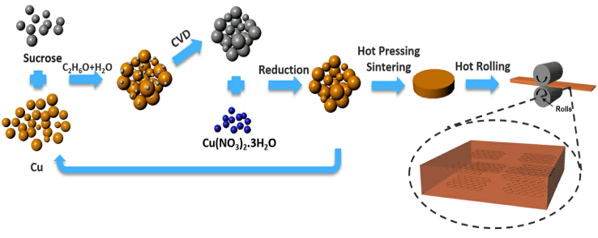
\includegraphics[width=\linewidth]{graphics/chapter_1/in_situ_growth}
\caption{Schematic illustration of the in-situ growth for graphene reinforced Cu composite (\cite{guo2020situ}).}
\label{fig:in_situ_growth}
\end{figure}


The in-situ processing technique is widely being used because of its simplicity and applicability. The fabrication of composites containing well-ordered (aligned) and uniformly dispersed graphene composites via in-situ method could be economically preferred option (\cite{kawk2019simple}). Various studies suggest that strength of materials can be increased without any compromise on their other properties such as thermal and electrical conductivities, corrosion resistance etc. Some researchers (\cite{chen2016fabrication, liu2017situ, guo2020situ}) introduced a simple two-step process which comprises simply two steps, i.e. powder compaction and CVD. The spaces in the compacted sample act as catalyst sites (template) for graphene growth during CVD. This method ensures not only uniform dispersion of graphene in matrix but also helps in the formation of three dimensionally interconnected network of graphene surrounding the grains of matrix (\cite{kawk2019simple}). In this way, this process has potential to improve mechanical, thermal, chemical and wear properties simultaneously.

Zhang et al. (\cite{zhang2020powder}) developed a powder-metallurgy based strategy for fabricating 3DiGr-Cu composites for high-performance advanced structural materials, which involves the rapid thermal annealing (RTA) in situ growth of three dimensionally interconnected network of graphene (3DiGr) on Cu powder. During CVD process, 3DiGr grown on the Cu powders is directly welded and thus construct a 3D interconnected graphene network in the composites due to the coefficient of thermal expansion (CTE)-mismatch related thermal stress between 3DiGr and Cu. In the constructed composites, the highly interconnected feature of 3DiGr could not only endow it with a much larger interfacial shear stress than 2D isolated graphene in the composites for achieving a much better load transfer strengthening capability and a remarkably higher strengthening efficiency, but also greatly reduce the electrons scattering in the interfacial areas and construct extensive conducting highways throughout the matrix for electrons transportation. As a result, the 3DiGr-Cu composite demonstrates superior mechanical properties, electrical and thermal conductivity simultaneously, which has the potential to satisfy many special applications such as lightweight macroscopic conductors and heat-sinks in electronics. Moreover, this feasible and scalable bottom-up concept to welding graphene into a continuous network architecture during powder consolidation can enable new paths to design 3D network structure constructed by 2D building blocks in the metal matrix composites without the ubiquitous restrictions of currently-used melting-related processing methods.

In our research, we proposed an in-situ growth route, which starts from CuNi powders by using a simple two-steps method. Thereby, the overall fabrication process of 3DiGr-CuNi or 3Di hBN-CuNi composites could be primarily divided into two steps. We followed this method for the synthesis of graphene or hBN reinforced CuNi composites and found outstanding results with regards to application and properties.

\subsection{Applications of Gr/hBN in MMCs}

\subsubsection{Mechanical Properties}

MMCs reinforced by 2D materials have shown excellent mechanical properties including yield strength, tensile strength, toughness etc. Chu et al. (\cite{chu2014enhanced}) found that Gr-Cu composite showed enhancement in yield strength and Young’s modulus upto 114\% and 37\%, respectively compared to unreinforced Cu. Chen et al. (\cite{chen2016fabrication}) investigated on in-situ grown graphene reinforced Cu matrix composites and found 177\% and 27.4\% enhancement in yield and tensile strength over pure copper. Similarly, various researchers have observed a substantial increment in mechanical properties of the metal matrix as shown in Table \ref{tab:table1}. Shu et al. (\cite{shu2019synergetic}) reported the improved mechanical properties of Cu/Ti3SiC2/C nanocomposites due to synergetic effect of graphene and hBN. There are several mechanisms which can explain the reinforcing effect of graphene (or hBN) which are given below:


\begin{table}[!htb]
\centering
\caption{Mechanical properties of graphene reinforced MMCs.}
\resizebox{\linewidth}{!}
{
\begin{tabular}{lll}
\hline
Processing method                            & \begin{tabular}[c]{@{}l@{}}Ultimate tensile strength (MPa)\\ (Compared to Cu)\end{tabular} & Reference           \\ \hline
MLM + SPS                                    & 319 (increase 25\%)                                                                        & \cite{li2015reduced}       \\
Sonication + Spark plasa sintering           & 131 (decrease 24\%)                                                                        & \cite{li2014highly}        \\
Ball milling + Equal speed rolling           & 315.1 (decrease 0.7\%)                                                                     & \cite{kim2014multi}        \\
A in-situ two-step process                   & 218 (increase 20\%)                                                                        & \cite{jo2019tensile}       \\
Sonication + Hot pressing                    & 271 (increase 18\%)                                                                        & \cite{tang2014enhancement} \\
Ball milling + Sparking plasma sintering     & 355                                                                                        & \cite{cui2014effect}       \\
In-situ growth + Hot pressing + Hot rolling  & 275 (increase 27\%)                                                                        & \cite{guo2020situ}         \\
Ball milling + In situ growth + Hot pressing & 274 (increase 27.4\%)                                                                      & \cite{chen2016fabrication} \\ \hline
\end{tabular}
}
\label{tab:table1}
\end{table}


\subsubsubsection{Load Transfer}
3DiGr or 3Di-hBN, having strong interfacial bonding to metal matrix can transfer the externally applied load. This network sustains the applied load as a whole instead of as isolated pieces of graphene or hBN layers. Therefore, overall strength of the reinforced composite is enhanced (\cite{chen2016fabrication}). Figure explains the role of 3DiGr in increasing the strength by mechanism of load transfer. When the composite is under stress, graphene sustains a certain part of load transferred from the matrix in the process of deformation. Since graphene has much higher strength than the matrix, the matrix fractures before than graphene. After the fracture of metal matrix, graphene is lengthened and an extra force is needed to achieve the complete fracture of graphene, which can be corroborated by the morphology of the fracture surface. The schematic diagram Figure \ref{fig:load_transfer} is also helpful to explain the improvement in elongation of graphene/Cu composite. 


\begin{figure}[!htb]
\centering
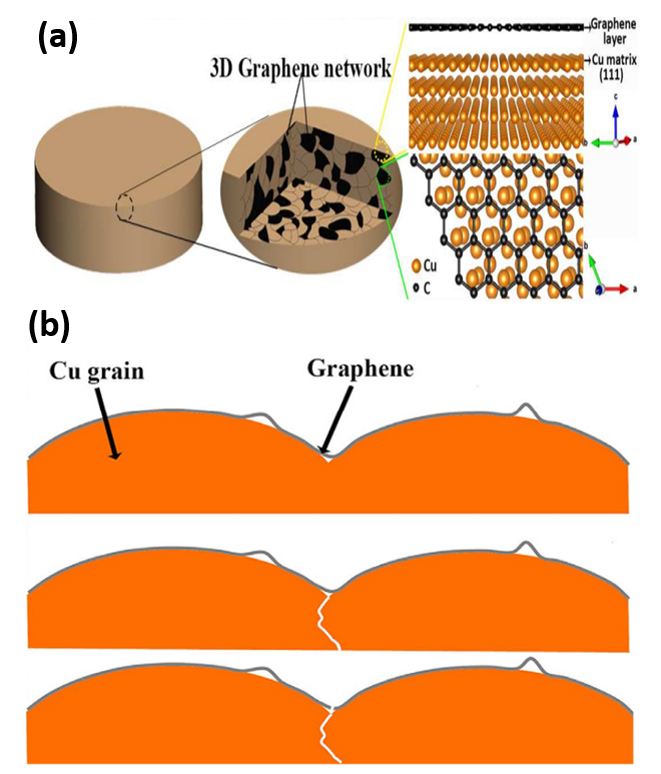
\includegraphics[scale=0.35]{graphics/chapter_1/load_transfer}
\caption{Schematic diagrams (a) 3DiGr (black areas) in Gr-Cu composite transferring the load in matrix(\cite{chu2018interface}) (b)Section view of graphene/Cu in the fracture process, the graphene delays the fracture under the mechanism of load transfer (\cite{chen2016fabrication}).}
\label{fig:load_transfer}
\end{figure}

\subsubsubsection{Dislocation Strengthening}
When external load is applied on the composite, the graphene or hBN can act as a barrier to inhibit the dislocation motion, leading to the dislocation accumulation nearby the interface (\cite{kim2013strengthening}). Chu et al. (\cite{chu2018interface}) explained that improved tensile properties of Gr-Cu composites can be attributed to the accumulation of dislocations at metal-graphene interfaces after tensile deformation, identified by transmission electron microscope (TEM) and X-ray diffraction (XRD) analyses.

\subsubsubsection{Grain refinement}
The inclusion of graphene or hBN in the metal matrix is quite likely to inhibit the grain growth during the synthesis process which leads to refinement in the structure (\cite{chu2014enhanced}). The grain size affects the yield and tensile strength of the sample according to the classic Hall-Petch equations (\cite{kato2014hall, zhang2017achieving}):

\begin{gather}
\label{eq:yield_strength}
\sigma_{YS}=\sigma_{YS}\ +\ k_{YS}d^{-1/2}
\\
\label{eq:ultimate_strength}
\sigma_{UTS}=\sigma_{UTS}\ +\ k_{UTS}d^{-1/2}
\end{gather}

where, $\sigma_{YS}$ and $\sigma_{UTS}$ correspond to the yield strength and the ultimate tensile strength, respectively. These equations indicate that the strength of a material increases with the decrease in grain size.

\subsubsection{Thermal properties}
Graphene has high thermal conductivity, so its inclusion in the metal matrix composite would increase the thermal conductivity. Zhang et al. (\cite{zhang2020powder}) found that three-dimensional network of graphene in Cu matrix contributed to more than 10\% increment in thermal conductivities. They explained their findings by conducting molecular dynamic simulations to prove that three-dimensional network of graphene provides effective conducting path channel for electrons and phonons motion. Li et al. (\cite{li2019thermal}) adopted a simple two-step process route to fabricate three dimensionally interconnected network of graphene Cu composite and found a substantial increase in thermal conductivity. Table summarizes the thermal conductivity of graphene reinforced Cu composites produced via various processing methods.

\begin{table}[!htb]
\centering
\caption{Thermal conductivities of graphene reinforced MMCs.}
\resizebox{\linewidth}{!}
{
\begin{tabular}{lll}
\hline
Processing methods                                                       & Thermal conductivity                                                                    & Reference               \\ \hline
Electrodeposition                                                        & 300.5 (increase 5\%)                                                                    & huang2016preparation    \\
MLM + SPS                                                                & \begin{tabular}[c]{@{}l@{}}P 362 (decrease 3\%)\\ P 345 (decrease 8\%)\end{tabular}     & chen2016effects         \\
Stirring + Hot pressing                                                  & 370 (increase 3\%)                                                                      & gao2016mechanical       \\
Pasting on Cu foil                                                       & 445.91 (increase 34\%)                                                                  & hsieh2017synthesis      \\
Direct deposition of graphene on Cu foil  Stacking
$+$SPS Ball milling$+$ SPS & 359 (increase 8\%)                                                                      & wejrzanowski2016thermal \\
In-situ two-step process                                                 & \begin{tabular}[c]{@{}l@{}}P 409 (increase 225\%)\\ P 385 (increase 208\%)\end{tabular} & li2019thermal           \\
Ball milling  Hot pressing                                               & 296 (increase 15\%)                                                                     & luo2017copper           \\
MLM  SPS                                                                 & 294 (decrease 18\%)                                                                     & si2017effect            \\
Ball milling  Hot pressing                                               & \begin{tabular}[c]{@{}l@{}}P 253\\ P 170\end{tabular}                                   & ponraj2017effect        \\
Sonication and vortex mixing  Vacuum infiltration  SPS                   & \begin{tabular}[c]{@{}l@{}}P 375 (increase 10\%)\\ P 150 (decrease 10\%)\end{tabular}   & chu2018thermal          \\ \hline
\end{tabular}
}
\label{tab:table2}
\end{table}

\subsubsection{Corrosion Properties}

One of the important applications of 2D materials is their ability to increase the corrosion resistance of MMCs. Graphene and hBN are impermeable to ions, molecules and atoms (\cite{mahvash2017corrosion}). Therefore, they can hamper the transfer of ions and molecules across the interface and increase the corrosion resistance of the composite. Mahveash et al. (\cite{mahvash2017corrosion}) reported that the CVD grown hBN reduces the Cu corrosion rate by an order of magnitude compared to bare Cu. Li et al. investigated the corrosion resistance of three-dimensionally interconnected networked graphene-Cu composite by potentiodynamic polarization tests and concluded that three-dimensional graphene structure effectively protected the Cu against corrosion. Because of impermeability, graphene or hBN does not let atomic hydrogen entering in the atomic structure and therefore can significantly enhance the resistance of metals and alloys to hydrogen embrittlement. Nam et al. (nam2014graphene) reported that graphene coating could be a protective barrier against the hydrogen embrittlement. Li et al., through the series of electrochemical experiment, also reported the higher tendency of three dimensionally interconnected graphene reinforced Cu composite to block the penetration of atomic hydrogen.

\subsection{Summary}
In summary, graphene and hBN has a large potential to reinforce the chemical, mechanical and thermal properties of metal matrix composites due to their outstanding properties. We found that there are several studies which discuss the properties of metal matrix composites reinforced by 3DiGr. However, a very limited amount of research has been done on the metal matrix composites reinforced by 3Di-hBN, despite the fact hBN has also has excellent mechanical, thermal and chemical properties. Therefore, in this dissertation, we particularly explored the applications of hBN in the CuNi matrix. We reported the mechanical, corrosive, high temperature oxidation, and thermal properties of 3Di-hBN reinforced CuNi composites fabricated by using a simple two-step process. Nevertheless, we also fabricated 3DiGr reinforced CuNi composite, and determined their scope to be used in the energy field. 





